\chapter{Usage Demonstration}
This chapter contains several demonstrations of the application of the library on practical problems with increasing difficulty. All of the presented examples are included in the library distribution package. To ensure that the mentioned results can be replicated, all instances of genetic algorithms use seeded entropy generators.

\section{Trivial Example}
The first example is a very trivial problem. It is defined as follows: \textit{Given all bit strings of length between 10 and 100 characters, find the string which maximizes the number of ones.} Although the optimal solution is clearly a string of 100 ones, the simplicity of the problem is ideally suited for demonstration of the individual components of the library.

\subsection{Chromosome and Fitness}
The domain space is a finite set. Its points can be characterized as range-initialized arrays of Boolean values with the initialization interval $[10;100]$, which is declared analogically to the array used in solving the Knapsack Problem (see Listing \ref{listing:array-knapsack}). Since range-initialized arrays already support basic genetic operators, they can be used as chromosomes in the GA.

To evaluate and compare the quality of chromosomes, a fitness function is required. For the purposes of this simple example, the fitness function can be defined as
~
\begin{align}
	f(s_1, s_2, \dots, s_{n}) = \frac{1}{100}\sum_{i=1}^{n} s_i
\end{align}
~
where $\{s_i\}_{i=1}^{n}$ are the bits and $n\in[10;100]$ is the length of the chromosome. A simple implementation of a sequential evaluator using this function is shown in Listing \ref{listing:evaluator-sequential-maxone}.

\begin{listing}[ht]
	\inputswift{evaluator-sequential-maxone}
	\caption{Example of a sequential evaluator for the MAX-ONE Problem.}
	\label{listing:evaluator-sequential-maxone}
\end{listing}

\subsection{Algorithm}
With both the chromosome data structure and the fitness function defined, the only remaining step is to declare and configure the instance of the GA before a run can be started. 

\begin{listing}[ht]
	\inputswift{algorithm-maxone}
	\caption{Example of the GA definition for the MAX-ONE Problem.}
	\label{listing:algorithm-maxone}
\end{listing}

To clearly explain the syntax of the \texttt{GeneticAlgorithm<T>} class initializer, the algorithm shown in Listing \ref{listing:algorithm-maxone} has the following properties:
~
\begin{itemize}
	\item The number of individuals in every generation is 200.
	\item Elitism is used to preserve the best chromosome.
	\item The algorithm terminates after 1000 iterations or after the highest fitness value reaches 1.0.
	\item The $\beta$-tree contains a single chance node:
	~
	\begin{itemize}
		\item With the probability 0.5, apply the reproduction operator on a random individual.
		\item With the probability 0.3, apply the mutation operator on an individual selected by the roulette selection.
		\item With the probability 0.2, apply the one-point crossover operator on the winners of two randomized tournaments, each containing five contestants.
	\end{itemize}
\end{itemize}

When executed, the presented algorithm performs 757~iterations before reaching the best fitness value~1.0 and yielding the optimal solution consisting of 100~ones. On the experimental computer\footnote{The experimental computer was Apple Mac mini (model \textit{Late 2012}) with Intel Core i7 CPU (2.3~GHz) and 8~GB RAM (1600~MHz DDR3).}, the evaluation of the algorithm took approximately 5.6~seconds.

To further increase its speed, it is possible to utilize parallelization of fitness evaluation as described in Section \ref{section:parallel-evaluators}. By substituting the line no. 13 of Listing \ref{listing:algorithm-maxone} with \mintinline{swift}{ParallelEvaluator() { _ in MaxOneEvaluator() }}, the library creates a separate evaluator instance for every CPU core, instead of sharing a single instance among all cores.

After this modification, the number of performed iterations remains the same, however, the total execution time decreases to 4.2~seconds. Note even though the experimental computer has 8 core CPU, such a small decrease in evaluation time is acceptable due to the fact that the only parallelized part of the algorithm is the evaluation of the fitness function, which in this particular case does not represent a significant portion of the processing time. The convergence of fitness values is plotted in Figure \ref{fig:maxone-fitness}.

\begin{figure}[ht]
	\centering
	\begin{tikzpicture}
		\begin{axis}[
			height=9cm,
			width=0.9\textwidth,
			grid=major,
			xlabel={Generation},
			ylabel={Fitness},
			ymin=0, ymax=1,
			xmin=1, xmax=757,
			no markers,
			legend pos=south east
		]
			
		\addplot table {data/maxone-fitness-best.dat};
		\addlegendentry{Best fitness}

		\addplot table {data/maxone-fitness-average.dat};
		\addlegendentry{Average fitness}

		\end{axis}
	\end{tikzpicture}
	\caption[MAX-ONE genetic algorithm fitness convergence chart.]{Fitness convergence chart of the GA from Listing \ref{listing:algorithm-maxone}.}
	\label{fig:maxone-fitness}
\end{figure}

\section{Self-driving Car Simulation}
The second example can be considered slightly more complex and closer to practical applications than the MAX-ONE Problem. Suppose that there is a robot car capable of navigating in a simulated two-dimensional environment, which contains a closed curve called the \textit{track}. The goal is to find a way to steer the car, so that its movements follow the track. In real-world applications, this goal would be equivalent to keeping a car within the bounds of the road.

The simulated car is controlled by two parameters: the \textit{steering} and the \textit{acceleration}. Modelled after physical driving control systems like the steering wheel and the accelerator pedal, changes of these parameters cannot influence the heading and the velocity of the car directly. Instead, the control parameters affect car's heading and velocity gradually with respect to time, behaving more like their first derivatives.

An event loop operates in the simulated environment, evaluating all variables periodically with a sufficient frequency. This event loop is responsible for altering the position of the car with respect to its instantaneous velocity and recalculating the instantaneous velocity with respect to the latest value of the acceleration control parameter. A similar process serves to adjust the heading of the car. However, while the acceleration is a continuous decimal parameter with values chosen within a set interval, the steering parameter is fundamentally a discrete choice between set values:
~
\begin{itemize}
	\item hard left,
	\item left,
	\item neutral,
	\item right,
	\item hard right.
\end{itemize}

To recognize the track in the environment, the robotic car is equipped with a set of simulated real-time detectors, which are positioned in a way to approximate the viewport of a real car driver. There are three detectors located in front of the car, one under the car and one behind it. All detectors are capable of producing Boolean values, signifying whether the closed curve is located on their exact position at the time of measurement. This configuration approximates thresholding techniques, which are frequently used in detectors of real self-driving car prototypes.

\subsection{Control Program}
The control program of the car is a dedicated real-time software, which periodically interacts with the event loop of the environment in order to determine the values of control parameters based on the outputs of the on-board detectors.

To demonstrate how the presented library can be used in conjunction with other Swift components, it was decided that the car is to be controlled by a three-layer feedforward neural network (for definition, see Section \ref{section:neural-networks}). The input layer of the network is comprised of 5 nodes corresponding to binary read-outs of the on-board detectors, the hidden layer contains 10 nodes and the output layer contains 2 nodes corresponding to the control parameters of the car.

While the acceleration parameter is directly equal\footnote{The acceleration parameter is artificially clamped to the $[-100;100]$ interval to mimic physical limitations of the car.} to the output of its respective node, the steering parameter uses thresholds to determine in which directions should the heading of the car be adjusted.

\subsection{Chromosome and Fitness}
By standard means, it is possible to encode every neural network described in the previous section as a real vector from $d$-dimensional space, where $d$ denotes the number of interunit connections and the components of the vector correspond to weight coefficients of such connections. By assuming that all connections between neurons from consecutive layers exist (substituting the weight 0 for non-existing connections), fixed length of the vector can be ensured. The neural network can be therefore characterized by a range-initialized array of real numbers with the initialization interval $[d;d]$. Accounting for 5, 10 and 2 neurons in the input, hidden and output layer respectively, $d=5\cdot 10+10\cdot 2=70$.

To evaluate and compare the quality of control programs, a simple simulated test is performed. Prior to the test, a random track is generated and positioned within the environment. The test is performed by placing the car on a random position with random orientation and executing its control program continuously for a set period of time. Throughout the test, various parameters of the car are monitored and recorded by the event loop. Should the car leavesthe bounds of the simulated environment at any instance, the test is terminated prematurely. After 3 randomized tests are performed, the fitness function of the control program is evaluated as
~
\begin{align}
	f(t_1,t_2,t_3) = \frac{t_1 + t_2 + t_3}{3 \cdot t_{max}}
\end{align}
~
where $t_{max}$ is the maximum duration of a single randomized test and $t_1,t_2,t_3$ denote sums of durations spent\footnote{As recorded by the detector under the car.} on the track by the car during tests 1, 2 and 3 respectively. All durations are specified in seconds.

Clearly, the presented fitness function favors control programs which manage to keep the car on the track more than programs which do not follow it very well or veer off it eventually. Of course, randomly driving over the track affects the final fitness value even though the control program might not manage to follow it. Nevertheless, performing the test multiple times with randomized parameters should minimize the probability of misclassification. An implementation of a sequential evaluator using this function is illustrated in Listing \ref{listing:evaluator-sequential-car}.

\begin{listing}[ht]
	\inputswift{evaluator-sequential-car}
	\caption{Implementation of the self-driving car evaluator.}
	\label{listing:evaluator-sequential-car}
\end{listing}

In the evaluator, the control program along with the neural network itself\footnote{The implementation of the FFNN was provided by the \textit{Swift AI} open-source project, which is available online: \url{https://github.com/collinhundley/Swift-AI}} is encapsulated in an instance of the \texttt{NetDriver} type, which is conformant to the \texttt{CarDriver} protocol that formalizes requirements on automated car controllers.

\todo % doplnit výsledek

\section{Automated QWOP Player}
The third and final usage demonstration of the presented library is closely related to genetic programming techniques proposed in \cite{EvolvingQwopGaits}. In the referenced publication, researchers describe their attempts at training artificial programs in playing an online computer game, achieving scores comparable to or exceeding those of human players. This section is dedicated to replicating parts of their results.

\subsection{The QWOP Game}
QWOP (shown in Figure \ref{figure:QWOP}) is a popular online game, available for free at Foddy.net. \cite{QwopWebsite} In the game, the player controls movements of an Olympic athlete during a sprint race. The objective is to reach the longest possible distance, terminating at the 100-meter mark. If at any point throughout the race the head or any of the hands of the athlete come into contact with the ground, the athlete loses his balance, falls and the game is over. The control scheme of QWOP is very simple. By pressing keys Q, W, O, P on the keyboard (hence the name of the game), the player controls movements of different muscle groups within the athlete's body. Keys Q and W move forward the left and the right thighs and keys O and P move backward the left and the right calves respectively.

\begin{figure}[ht]
	\centering
	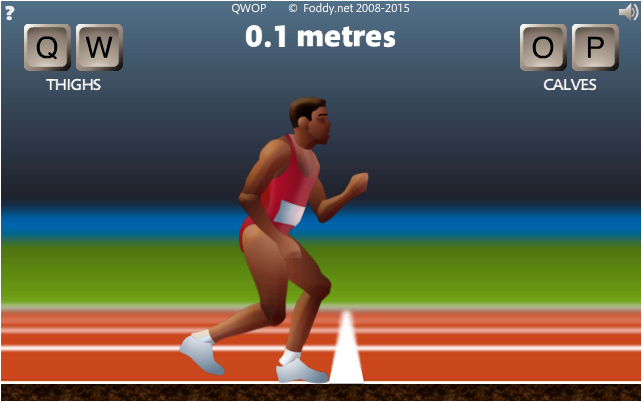
\includegraphics[width=0.8\textwidth]{img/qwop.png}
	\caption[The QWOP online game.]{The QWOP online game. \cite{QwopWebsite}}
	\label{figure:QWOP}
\end{figure}

In spite of the simplicity of the game goals and the straightforward control scheme, QWOP is well-known for its notorious difficulty. This is mainly due to its ``ragdoll physics'' engine, which heavily oversimplifies the mechanics of th simulated runner to the point where certain behaviors might seem unintuitive or even unpredictable. \cite{QwopHomework} The biggest challenge of the game can be described as to devise a repeatable strategy to achieve and maintain precise synchronization of key presses, receiving only limited sensory feedback from the game.

\subsection{Previous Work}
QWOP has been mentioned in several publications, mostly in relation to machine learning. The challenge of the game has been subject of study primarily because of its appearent similarity to the problem of evolving bipedal gaits in physical robots and other cybernetic applications.

To describe QWOP strategies, the authors of \cite{EvolvingQwopGaits} have used string encodings. Since one of these encodings is used\footnote{The used encoding is the \textit{Encoding 1}, which was originally proposed by \cite{QwopEncoding}.} in this demonstration, its definition is included in this section. The encoded strings represent sequences of instructions to the player without any regards to the state of the game. The encoding uses symbols ``\texttt{q,Q,w,W,o,O,p,P,+}''. A capital letter represents pressing the corresponding key on the keyboard, a lowercase letter represents a key release. The ``\texttt{+}'' symbol stands for a delay in which the current state of inputs is maintained for 150 milliseconds. \cite{EvolvingQwopGaits}

Upon interpretation, the encoded string is read from the left to the right, executing one instruction at a time. When the end of the string is reached, the interpretation starts again from the beginning. An example of a strategy encoded in this way is shown in Listing \ref{listing:encoding-example}.

\begin{listing}[ht]
	\begin{minted}[frame=lines,
               framesep=2mm,
               fontsize=\small]{text}
QO+qPW+wpo+QPW+wO+qp+P+Q+++qp+QPW+wo+qp+POQ+q+W+Qp+qwo
	\end{minted}
	\caption[Example encoded QWOP game strategy.]{Example encoded QWOP game strategy, which translates to \textit{``Press Q and O, hold them for 150ms, release Q, press P and W, hold for 150ms, release W, P and O, wait...''} \cite{EvolvingQwopGaits}}
	\label{listing:encoding-example}
\end{listing}

To consistently interpret QWOP strategies encoded into strings, the authors of \cite{EvolvingQwopGaits} have used automated Java program called the \textit{Qwopper}, which has been originally developed by \cite{QwopEncoding}. The application is comprised of three components:
~
\begin{description}
	\item[Strategy interpretter]
	The interpretter is responsible for creating artificial user inputs for the QWOP game in compliance with a given strategy string.

	\item[Control interface]
	The control interface is a user application, which serves users to configure and test the interpretter.

	\item[GA engine]
	By default, Qwopper includes its own implementation of the GA, which has been used to produce strings by means of genetic programming.
\end{description}

Apart from blindly simulating user inputs, the interpretter component of Qwopper includes a basic OCR algorithm (illustrated in Figure \ref{figure:QWOP-OCR}), which is capable of determining the current state of the game (\textit{running} or \textit{paused}) and the distance traveled by the athlete. Combining this information with the duration of the interpretation, Qwopper can periodically estimate the instantaneous velocity of the runner achieved by a given strategy.

\begin{figure}[ht]
	\centering
	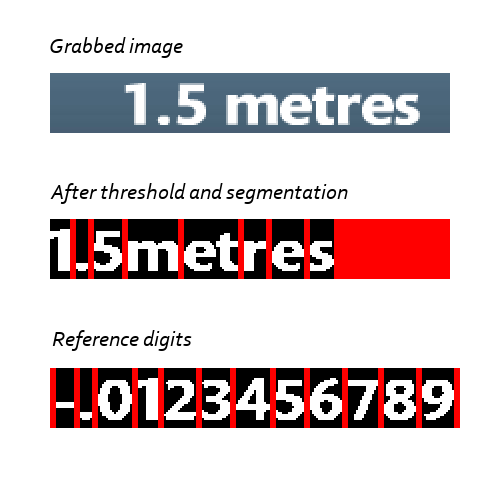
\includegraphics[width=0.5\textwidth]{img/reading_digits.png}
	\caption[OCR process used by the Qwopper software.]{Illustration of the OCR process used by the Qwopper software. \cite{QwopEncoding}}
	\label{figure:QWOP-OCR}
\end{figure}

It is worth noting at this point that Qwopper already has all necessary components to generate, evaluate and recombine QWOP strategy strings on its own. However, for the purpose of demonstration of the presented library, its functions are reduced to only serve as a strategy string evaluation tool.

\subsection{Interfacing Qwopper with Swift}
asd
